%%%%%%%%%%%%%%%%%%%%%%%%%%%%%%%%%%%%%%%%%
% Wenneker Article
% LaTeX Template
% Version 2.0 (28/2/17)
%
% This template was downloaded from:
% http://www.LaTeXTemplates.com
%
% Authors:
% Vel (vel@LaTeXTemplates.com)
% Frits Wenneker
%
% License:
% CC BY-NC-SA 3.0 (http://creativecommons.org/licenses/by-nc-sa/3.0/)
%
% Adapted for COMS30007 by Carl Henrik Ek
%
%%%%%%%%%%%%%%%%%%%%%%%%%%%%%%%%%%%%%%%%%

%----------------------------------------------------------------------------------------
%	PACKAGES AND OTHER DOCUMENT CONFIGURATIONS
%----------------------------------------------------------------------------------------

\documentclass[10pt, a4paper, twocolumn]{article} % 10pt font size (11 and 12 also possible), A4 paper (letterpaper for US letter) and two column layout (remove for one column)

%%%%%%%%%%%%%%%%%%%%%%%%%%%%%%%%%%%%%%%%%
% Wenneker Article
% Structure Specification File
% Version 1.0 (28/2/17)
%
% This file originates from:
% http://www.LaTeXTemplates.com
%
% Authors:
% Frits Wenneker
% Vel (vel@LaTeXTemplates.com)
%
% License:
% CC BY-NC-SA 3.0 (http://creativecommons.org/licenses/by-nc-sa/3.0/)
%
% Adapted for COMS30007 by Carl Henrik Ek
%
%%%%%%%%%%%%%%%%%%%%%%%%%%%%%%%%%%%%%%%%%

%----------------------------------------------------------------------------------------
%	PACKAGES AND OTHER DOCUMENT CONFIGURATIONS
%----------------------------------------------------------------------------------------

\usepackage[english]{babel} % English language hyphenation

\usepackage{microtype} % Better typography

\usepackage{amsthm} % Math packages for equations
\usepackage{amsmath}
\usepackage{amssymb}
\usepackage{mathtools}
\usepackage{bm}
\usepackage{xfrac}
\usepackage{resizegather}



\usepackage[svgnames]{xcolor} % Enabling colors by their 'svgnames'

\usepackage[hang, small, labelfont=bf, up, textfont=it]{caption} % Custom captions under/above tables and figures

\usepackage{booktabs} % Horizontal rules in tables

\usepackage{lastpage} % Used to determine the number of pages in the document (for "Page X of Total")

\usepackage{graphicx} % Required for adding images

\usepackage{enumitem} % Required for customising lists
\setlist{noitemsep} % Remove spacing between bullet/numbered list elements

\usepackage{sectsty} % Enables custom section titles
\allsectionsfont{\usefont{OT1}{phv}{b}{n}} % Change the font of all section commands (Helvetica)

%----------------------------------------------------------------------------------------
%	MARGINS AND SPACING
%----------------------------------------------------------------------------------------

\usepackage{geometry} % Required for adjusting page dimensions

\geometry{
	top=1cm, % Top margin
	bottom=1.5cm, % Bottom margin
	left=2cm, % Left margin
	right=2cm, % Right margin
	includehead, % Include space for a header
	includefoot, % Include space for a footer
	%showframe, % Uncomment to show how the type block is set on the page
}

\setlength{\columnsep}{7mm} % Column separation width

%----------------------------------------------------------------------------------------
%	FONTS
%----------------------------------------------------------------------------------------

\usepackage[T1]{fontenc} % Output font encoding for international characters
\usepackage[utf8]{inputenc} % Required for inputting international characters

\usepackage{XCharter} % Use the XCharter font

%----------------------------------------------------------------------------------------
%	HEADERS AND FOOTERS
%----------------------------------------------------------------------------------------

\usepackage{fancyhdr} % Needed to define custom headers/footers
\pagestyle{fancy} % Enables the custom headers/footers

\renewcommand{\headrulewidth}{0.0pt} % No header rule
\renewcommand{\footrulewidth}{0.4pt} % Thin footer rule

\renewcommand{\sectionmark}[1]{\markboth{#1}{}} % Removes the section number from the header when \leftmark is used

%\nouppercase\leftmark % Add this to one of the lines below if you want a section title in the header/footer

% Headers
\lhead{} % Left header
\chead{\textit{\thetitle}} % Center header - currently printing the article title
\rhead{} % Right header

% Footers
\lfoot{} % Left footer
\cfoot{} % Center footer
\rfoot{\footnotesize Page \thepage\ of \pageref{LastPage}} % Right footer, "Page 1 of 2"

\fancypagestyle{firstpage}{ % Page style for the first page with the title
	\fancyhf{}
	\renewcommand{\footrulewidth}{0pt} % Suppress footer rule
}

%----------------------------------------------------------------------------------------
%	TITLE SECTION
%----------------------------------------------------------------------------------------

\newcommand{\authorstyle}[1]{{\large\usefont{OT1}{phv}{b}{n}\color{DarkRed}#1}} % Authors style (Helvetica)

\newcommand{\institution}[1]{{\footnotesize\usefont{OT1}{phv}{m}{sl}\color{Black}#1}} % Institutions style (Helvetica)

\usepackage{titling} % Allows custom title configuration

\newcommand{\HorRule}{\color{DarkGoldenrod}\rule{\linewidth}{1pt}} % Defines the gold horizontal rule around the title

\pretitle{
	\vspace{-30pt} % Move the entire title section up
	\HorRule\vspace{10pt} % Horizontal rule before the title
	\fontsize{32}{36}\usefont{OT1}{phv}{b}{n}\selectfont % Helvetica
	\color{DarkRed} % Text colour for the title and author(s)
}

\posttitle{\par\vskip 15pt} % Whitespace under the title

\preauthor{} % Anything that will appear before \author is printed

\postauthor{ % Anything that will appear after \author is printed
	\vspace{10pt} % Space before the rule
	\par\HorRule % Horizontal rule after the title
	\vspace{20pt} % Space after the title section
}

%----------------------------------------------------------------------------------------
%	ABSTRACT
%----------------------------------------------------------------------------------------

\usepackage{lettrine} % Package to accentuate the first letter of the text (lettrine)
\usepackage{fix-cm}	% Fixes the height of the lettrine

\newcommand{\initial}[1]{ % Defines the command and style for the lettrine
	\lettrine[lines=3,findent=4pt,nindent=0pt]{% Lettrine takes up 3 lines, the text to the right of it is indented 4pt and further indenting of lines 2+ is stopped
		\color{DarkGoldenrod}% Lettrine colour
		{#1}% The letter
	}{}%
}

\usepackage{xstring} % Required for string manipulation

\newcommand{\lettrineabstract}[1]{
	\StrLeft{#1}{1}[\firstletter] % Capture the first letter of the abstract for the lettrine
	\initial{\firstletter}\textbf{\StrGobbleLeft{#1}{1}} % Print the abstract with the first letter as a lettrine and the rest in bold
}

%----------------------------------------------------------------------------------------
%	BIBLIOGRAPHY
%----------------------------------------------------------------------------------------

\usepackage[backend=bibtex,style=authoryear]{biblatex} % Use the bibtex backend with the authoryear citation style (which resembles APA)

\addbibresource{example.bib} % The filename of the bibliography

\usepackage[autostyle=true]{csquotes} % Required to generate language-dependent quotes in the bibliography
 % Specifies the document structure and loads requires packages

\usepackage{lipsum}
\usepackage{caption}
\usepackage{subcaption}

%----------------------------------------------------------------------------------------
%	ARTICLE INFORMATION
%----------------------------------------------------------------------------------------

\title{Models} % The article title

\author{
	\authorstyle{Justin Salmon\textsuperscript{1} and George Lancaster\textsuperscript{2}} % Authors
	\newline\newline % Space before institutions
	\textsuperscript{1}\institution{wr18313}\\ % Institution 1
	\textsuperscript{2}\institution{qv18258} % Institution 2
}


\date{\today} % Add a date here if you would like one to appear underneath the title block, use \today for the current date, leave empty for no date

%----------------------------------------------------------------------------------------

\begin{document}

\maketitle % Print the title

\thispagestyle{firstpage} % Apply the page style for the first page (no headers and footers)

%----------------------------------------------------------------------------------------
%	ABSTRACT
%----------------------------------------------------------------------------------------
\lettrineabstract{Abstract}

%----------------------------------------------------------------------------------------
%	ARTICLE CONTENTS
%----------------------------------------------------------------------------------------

\section{The Prior}

\subsection{Theory}

\subsubsection*{Question 1.1}
A Gaussian likelihood encodes the inherent noise present in most real-world data. The central limit theorem states that in most cases, when independent random variables are added and normalised, the result is a gaussian distribution. In other words, most probabilistic processes in nature tend to be noisy, and that noise tends to follow a Gaussian distribution. Hence this is generally a good first assumption to make about unknown data.
%Noise in input data - assume noise is gaussian -> implies gaussian likelihood
\subsubsection*{Question 1.2}
Choosing a spherical covariance matrix means that we are assuming that the distribution is equally likely to deviate from the mean in all directions. Additionally, we assume that all dimensions of \emph{y} are independent, and therefore do not covary with one another. Again, this is a good place to start. \par
Choosing a non-spherical covariance would imply that we know something in advance about the relationship between the different dimensions of \emph{y}.

% *input and output, which is not true in this case.

\subsubsection*{Question 2}
The covariance matrix would not be in terms of the identity matrix. We would have non-zero values in the offset diagonals which correspond to the correlations between different variables. If we apply the product rule, 

\subsubsection{Linear Regression}

\subsubsection*{Question 3}

\begin{align}
  p(\mathbf{Y} | \mathbf{X}, \mathbf{W}, \beta) = \prod_{i=0}^N \mathcal{N} (y_i | \mathbf{W}^T\phi(x_i), \beta^-1)
\end{align}

\subsubsection*{Question 4}

A distribution is conjugate to another if they both take the same algebraic form, meaning that they are in the same probability distribution family. For example, Gaussians are conjugate to each other, and the conjugate to a Bernoulli distribution is a Beta distribution. Conjugates are used as a convenience to avoid calculating the denominator in Baye's rule (the evidence) which can often be an integral. If the prior and likelihood are conjugate, then their product will be proportional to the posterior.

%A conjugate prior can simplify the equations for sampling. A gaussian prior is conjugate to to the likelihood function

\subsubsection*{Question 5}

Euclidean distance from the mean
X appears only in the gaussian exponential part
Euclidean distance because of spherical covariance? 

\subsubsection*{Question 6}

Derive posterior mean and covariance, start at conjugacy. Watch video https://www.youtube.com/watch?v=nrd4AnDLR3U

\subsubsection{Non-parametric Regression}

\subsubsection*{Question 7}

Non-parametric models are not focused on defining a set of parameters, but using what we know about the current data to classify new unseen data points. The data can be seen as analogous to the parameters. A good example of this is the K-nearest-neighbor model, which classifies new data points based on its surrounding classes. Unlike parametric models, non-parametric models do not assume that there is a finite set of parameters. Because of this, their complexity is not bounded by the number of parameters. 
\par
Non-parametric models may be more difficult to interpret as they do not have direct parameters to describe the model. 

\subsubsection*{Question 8}

This prior represents the space of all possible functions, however we want this to be constrained by making some functions more likely than others. The covariance $ k(\mathbf{X}, \mathbf{X})$ allows us to assume that any two values $x_i$ and $x_j$ covary, therefore $f_i$ and $f_j$ can also be expected to covary. This means that we think that smooth functions are more likely, however the probability of saw-tooth functions are non-zero.

\subsubsection*{Question 9}

All functions are possible, however some are more likely than others. 

\subsubsection*{Question 10}

\begin{align}
  p(\mathbf{Y},\mathbf{X}, f, \mathbf{\theta}) = p(Y|f)p(F|X,\theta)p(X)p(\theta)
\end{align}

\begin{figure}[htbp]
\centerline{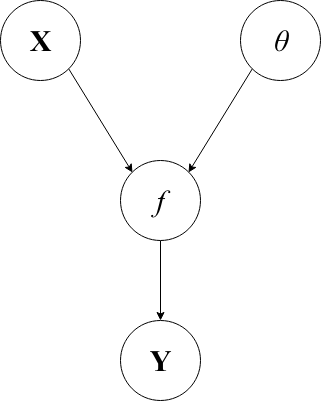
\includegraphics[width=0.5\linewidth]{question_10.png}}
\caption{Graphical model of the joint distribution.}
\label{fig2}
\end{figure}

\begin{itemize}
\item $\mathbf{X}$ and $\theta$ do not depend on anything;
\item $\mathbf{F}$ depends on $\theta$ and $\mathbf{X}$;
\item $\mathbf{Y}$ depends on $\mathbf{F}$, but is is conditionally independent of $\mathbf{X}$ and $\theta$.
\end{itemize}
\subsubsection*{Question 11}

The marginalisation in Eq. 2 connects the prior and the data because we now have a way to directly generate $\mathbf{Y}$  values given $\mathbf{X}$ and $\theta$ value without knowing the actual form of $f$.
\par
Because we are uncertain about $f$, when we marginalise it out, the uncertainty gets pushed onto $\mathbf{Y}$.
\par
The fact that $\mathbf{\theta}$ is left on the left hand side of the expression after marginalisation means that it is needed, with $\mathbf{x}$, to calculate $\mathbf{Y}$. This implies that $\mathbf{Y}$ is dependent on theta.

\begin{figure}[htbp]
\centerline{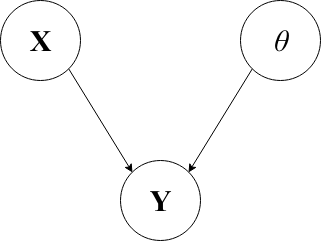
\includegraphics[width=0.5\linewidth]{question_11.png}}
\caption{Graphical model of the marginalised distribution.}
\label{fig2}
\end{figure}

%Use the model diagram to help?
%Marginalisation is the average of some distributions
%It is a weighted average of some functions, based on how likely each function is
\subsection{Practical}
\subsubsection{Linear Regression}
\subsubsection*{Question 12.1}

\begin{figure}[!htb]
\centerline{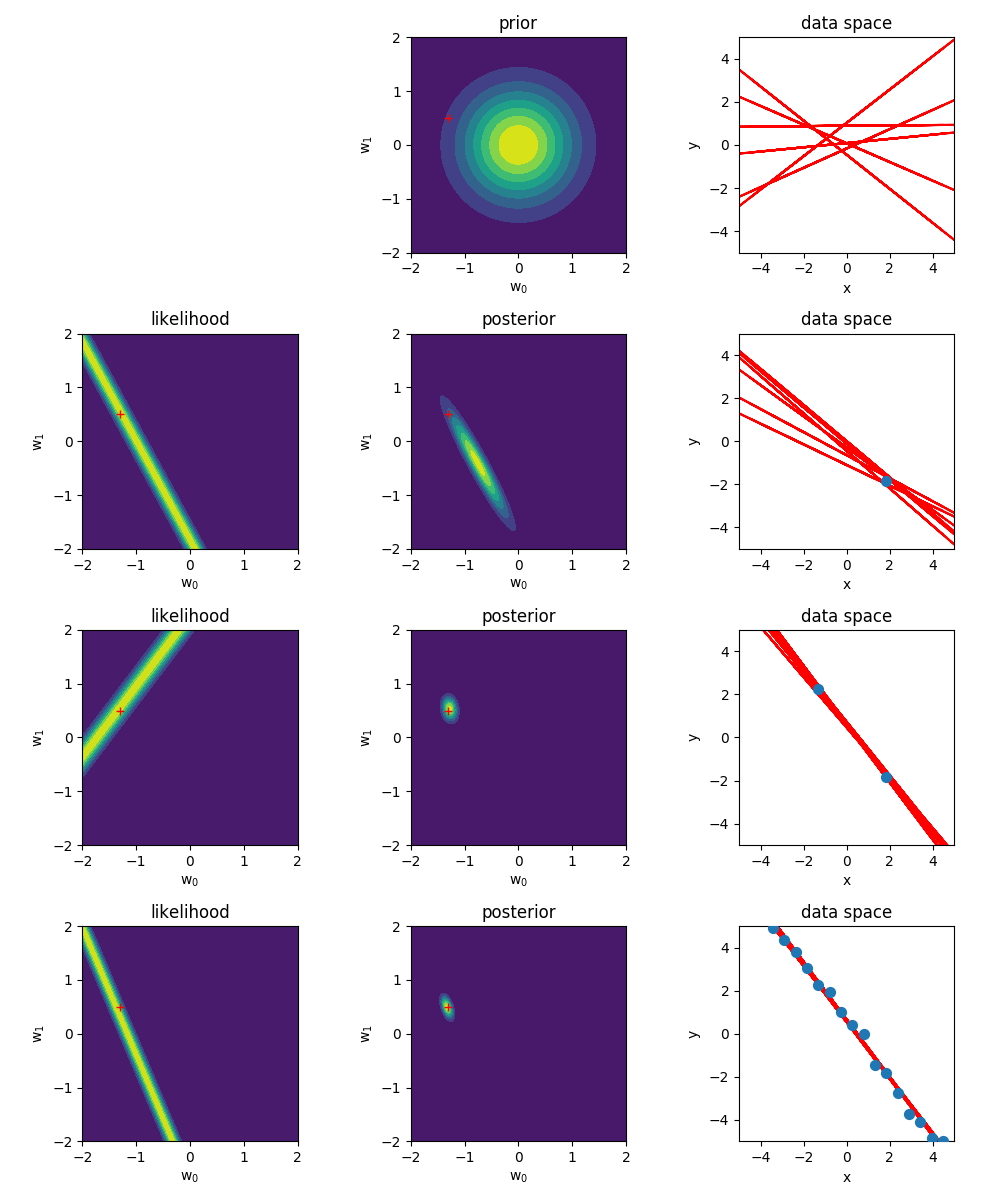
\includegraphics[width=\linewidth]{q12.png}}
\caption{Implementation of linear regression. The left hand column plots the likelihood. The middle column plots the prior/posterior, and the right hand column shows six random sample functions. Plots are drawn after one, two and twenty data points are revealed.}
\label{fig2}
\end{figure}

\subsubsection*{Question 12.5}
After a single data point is added, we can see that the posterior distribution begins to squash in one direction to converge onto the parameters $\mathbf{W}$. When we sample from this distribution, there are many lines passing through the point at different gradients, which is because we cannot define two parameters from a single data point. As we begin to reveal more data, the posterior distribution centres onto $\mathbf{W}$ and the sample functions fit more closely to the data points. This is a desirable behaviour as it shows that we have relearned the parameters of the model used to generate the data $\mathbf{X}$.
\subsubsection*{Question 12.6}
The posterior converges on the position of $\mathbf{W}$ because... 
\subsubsection*{Question 13}

\begin{figure}[!htb]
\centering
\begin{subfigure}{.5\linewidth}
  \centering
  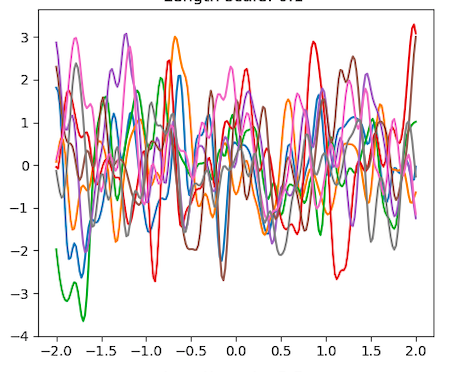
\includegraphics[width=.9\linewidth]{ls01.png}
  \caption{Length-scale of 0.1.}
  \label{fig:sub1}
\end{subfigure}%
\begin{subfigure}{.5\linewidth}
  \centering
  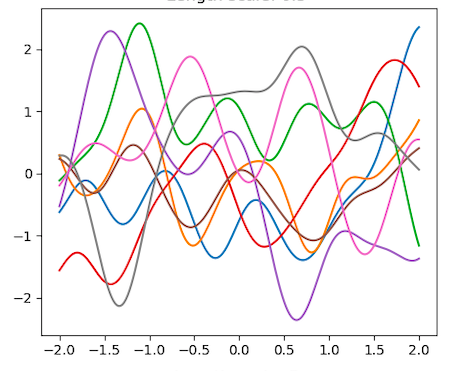
\includegraphics[width=.9\linewidth]{ls05.png}
  \caption{Length-scale of 0.5.}
  \label{fig:sub2}
\end{subfigure}
\begin{subfigure}{.5\linewidth}
\centering
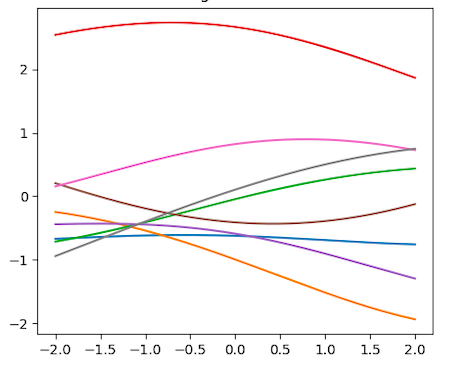
\includegraphics[width=0.9\linewidth]{ls5.png}
\caption{Length-scale of 5}
\end{subfigure}
\caption{Squared exponential with varying length scales. }
\label{fig:test}
\end{figure}

\subsubsection*{Question 13.4}
Increasing the length-scale of the covariance function allows us to constrain the functions smoothness. A smaller length-scale creates  functions with more rapid changes than those with a larger length-scale. This is because a higher length-scale means that, for two random variables $x_i$ and $x_j$ where the covariance is $k(x_i, x_j)$, their instantiations as $f_i$ and $f_j$ are similar. 
The samples in Fig 5 
\subsubsection{Question 14}
Need to describe the plots. What happens if we use a diagonal covariance matrix to the squared exponential. 
\begin{figure}[!htb]
\centerline{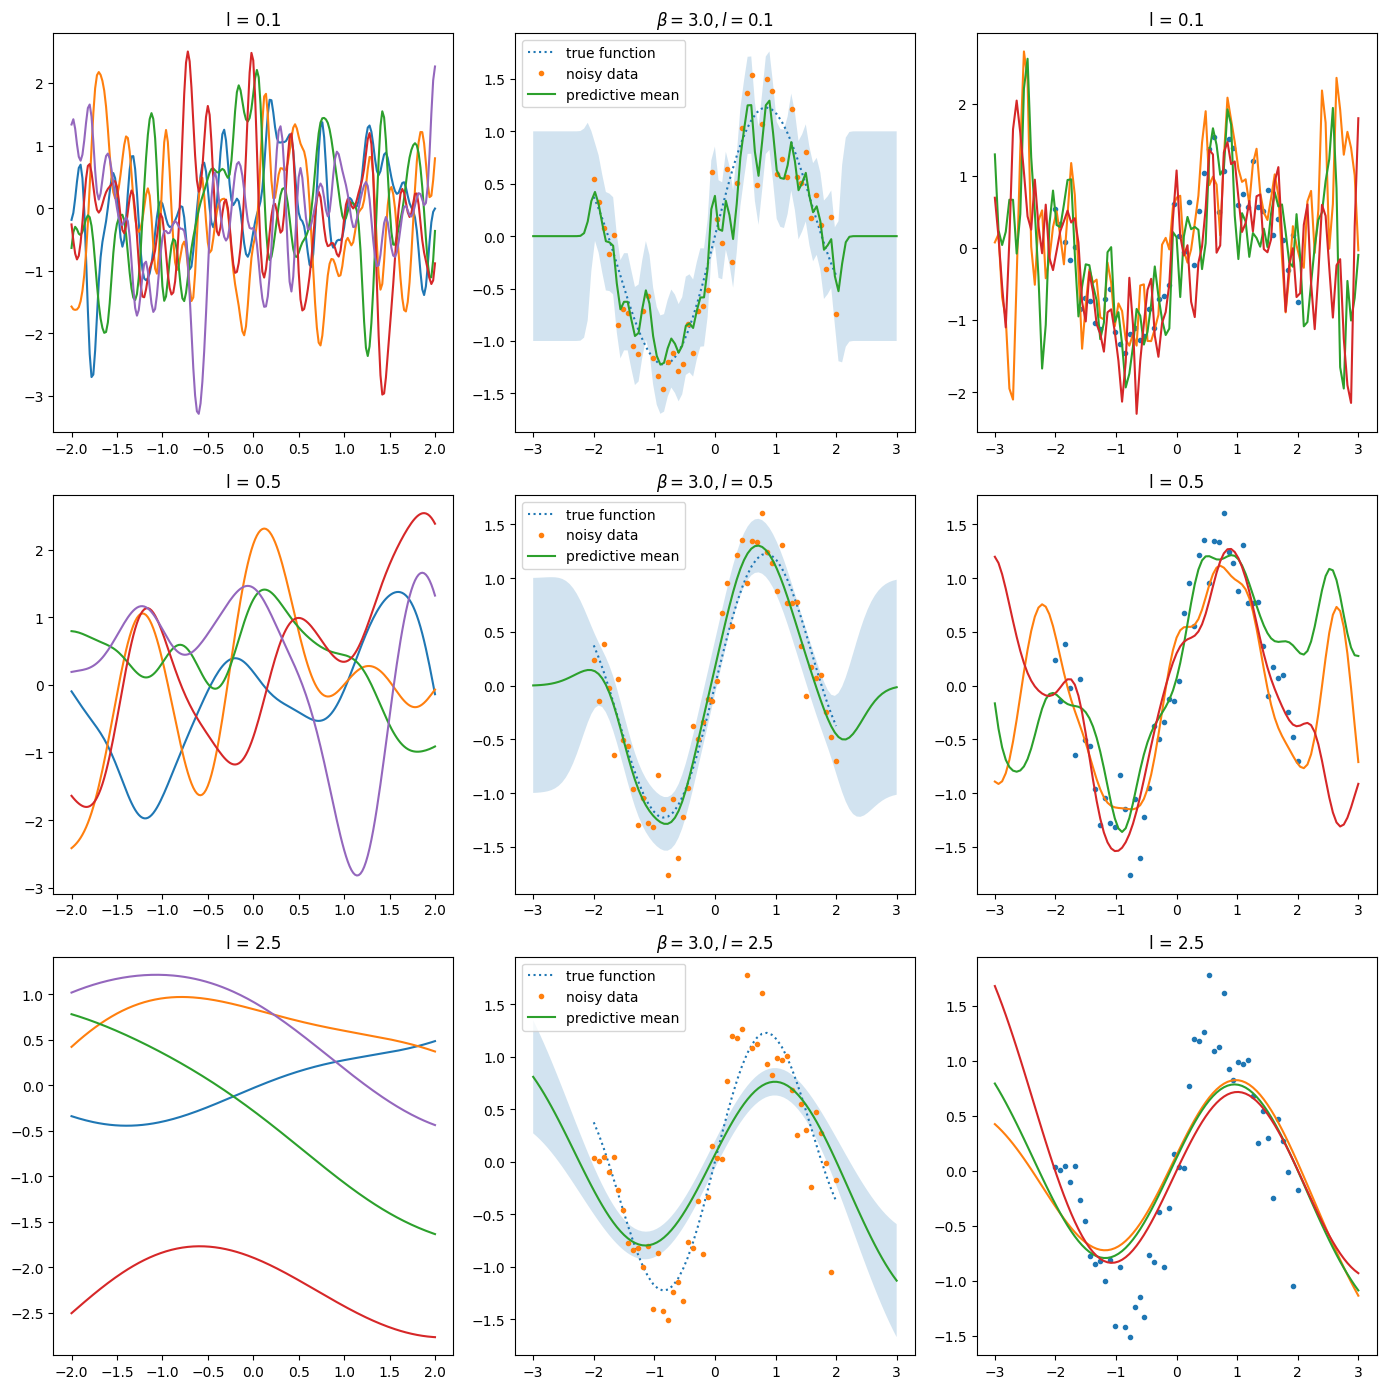
\includegraphics[width=\linewidth]{non_parametric_regression.png}}
\caption{Implementation of non-parametric regression with changing length-scales. }
\label{fig2}
\end{figure}

\section{Posterior}

\subsubsection*{Question 15}
We use our beliefs to find a starting point for the problem and to make assumptions about the data, or any other characteristics of the problem. Assumptions are what we assume to be true about something. If we had all the data we required for a problem, there would be no need to assume anything. This gives us a way to reason when we have very little information. \par
A preference is an assumption that we want to use because it is easier to do so. For example using a gaussian likelihood so that the posterior is also gaussian. -

We use beliefs and assumptions to formulate a prior. Believe that the smooth lines are more likely. Prefer straight or flat lines.

\subsubsection*{Question 16}

Since the covariance matrix is spherical, we have assumed that the latent input variables are independent and that they are centred around the origin. 

\subsubsection*{Question 17}

Look at the Gaussian Identities document to try to outline the steps to integrate out the variable we are not interested in

\subsubsection*{Question 18.1}
A maximum-a-posteriori (MAP) estimation is equal to the mode of the posterior. MAP finds the parameters that maximise the posterior distribution. \par
The maximum likelihood (ML) assumes a uniform prior distribution of the parameters. It finds the parameters that maximise the likelihood. 

%The prior is included in MAP, while ML only includes the likelihood. MAP takes both prior and likelihood into account.
%https://wiseodd.github.io/techblog/2017/01/01/mle-vs-map/

\subsubsection*{Question 18.2}
With only one data point, ML will be less accurate than MAP since it does not take the prior into account. However as more data is seen, the two will begin to converge on one another. 

\subsubsection*{Question 18.3}
The denominator has no bearing on argmax w becuase the integral is constant with respect to $\mathbf{W}$
Because the denominator equals one? The integral of the posterior equals one?

\subsubsection*{Question 19}
Not sure.

\subsubsection*{Question 20}
The uncertainty in $\mathbf{X}$ and $\theta$ is pushed into $f$. (not 100\% sure). 

\subsubsection*{Question 21}

\subsubsection*{Question 22}

\section{The Evidence}

%----------------------------------------------------------------------------------------
%	BIBLIOGRAPHY
%----------------------------------------------------------------------------------------

\printbibliography[title={Bibliography}] % Print the bibliography, section title in curly brackets

%----------------------------------------------------------------------------------------

\end{document}
